\chapter{Ambiente di Analisi}
Al fine di osservare il comportamento di SFA, e condurre l'analisi oggetto della Tesi, \`e stato costruito un ambiente atto a monitorare, in modo non intrusivo, il comportamento dell'algoritmo. \cite{monitoring}\\*
L'ambiente di analisi riproduce l'architettura software descritta nel capitolo 3, su una piattaforma \texttt{x86} equipaggiata con il sistema operativo \texttt{Windows 7}. 
\section{Principi di base}
L'ambiente di analisi deve essere tale da rispettare i principi della medesima. Non c'\`e interesse, nella fattispecie, a osservare il sistema a \emph{runtime}, ma lo scopo \`e unicamente quello di osservare il comportamento di SFA al variare dei dati in ingresso e dei parametri di configurazione.\\*
L'intero processo di analisi viene condotto attraverso un software appositamente realizzato, il \emph{Rail Track Tool} (RTT).\\*
Vengono escluse dalle campagne di analisi l'acquisizione delle misure dai sensori e la trasmissione degli output di SFA verso OBCU.\\*
Il sistema di acquisizione e trasmissione delle misure viene opportunamente \emph{mockato} \cite{mocking} da un insieme di classi di RTT che simulano il comportamento dei sensori.\\*
Le uscite di SFA vengono opportunamente visualizzate all'interno di RTT e al termine di ciascun esperimento viene prodotto un report \texttt{HTML}.
\section{Rail Track Tool}
RTT \`e un software \emph{front-end} realizzato al fine di valutare le performance di SFA.\\*
La sua architettura interna riproduce l'architettura software nominale del sistema di posizionamento.
Come \emph{listener}, RTT include tra le sue dipendenze la libreria \emph{SensorFusionLib}, e ne sfrutta le relative \texttt{API} per alimentare SFA ed ottenere gli output dell'algoritmo.\\*
\begin{figure}[h]
	\centering
	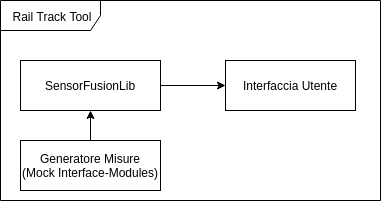
\includegraphics[width=0.7\linewidth]{img/RTTSchemaEasy}
	\caption{Architettura di analisi}
	\label{fig:rtteasy}
\end{figure}
\subsection{Interfaccia Utente}
All'avvio di RTT viene mostrata una finestra contenente l'interfaccia del software verso l'utente.
\begin{figure}[h]
	\centering
	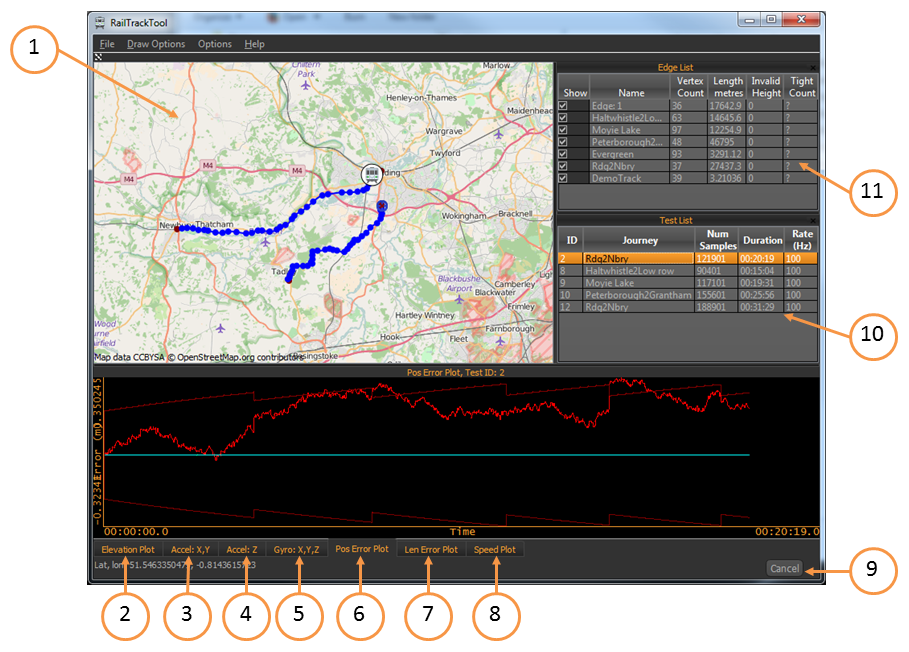
\includegraphics[height=8.2cm]{img/rtthci}
	\caption{Interfaccia RTT}
	\label{fig:rtt}
\end{figure}\newpage
Gli elementi che compongono tale interfaccia sono:
\begin{enumerate}
\item \texttt{Slippy map}: Mappa che visualizza le traccie memorizzate, all'interno delle quali verr\`a mostrata la posizione del treno durante l'esecuzione di SFA;
\item \texttt{Elevation plot}: Grafico che mostra l'altitudine della traccia in funzione della progressiva chilometrica della stessa;
\item \texttt{Accel X,Y}: Grafico delle misure dell'accelerometro fornite a SFA, relative agli assi normale e tangenziale alla traccia selezionata;
\item \texttt{Accel Z}: Grafico delle misure dell'accelerometro fornite a SFA, relative all'asse verticale alla traccia selezionata; 
\item \texttt{Gyro X,Y,Z}: Grafico delle misure del giroscopio fornite a SFA, relative agli assi normale, tangenziale e verticale alla traccia selezionata;
\item \texttt{Pos error plot}: Grafico che riporta, in funzione del tempo, la stima dell'errore commesso nel predire la posizione del treno;
\item \texttt{Len error plot}: Come \texttt{Pos error plot}, ma l'errore \`e espresso rispetto alla progressiva chilometrica e non rispetto al vettore posizione;
\item \texttt{Speed Plot}: Grafico che mostra la stima della velocit\`a del treno come funzione del tempo;
\item \texttt{Cancel button}: Pulsante da premere se si ha la necessit\`a di interrompere una simulazione;
\item \texttt{Test List}: Storico delle analisi effettuate;
\item \texttt{Edge List}: Lista delle tracce memorizzate.
\end{enumerate}
\subsection{Monitoring con RTT}
Tramite un'apposita interfaccia interna a RTT, l'utente ha la possibilit\`a di definire le caratteristiche dei sensori, come mostrato nelle figure \ref{fig:datagenerationconfig} e \ref{fig:imuconfig}. Definiti i parametri di configurazione \`e possibile selezionare una traccia, e simulare l'esecuzione di SFA.\\* Durante la simulazione, la posizione del treno stimata dall'algoritmo verr\`a visualizzare sulla mappa. 
\begin{figure}[h]
	\centering
	\includegraphics[width=0.7\linewidth]{../Trainpositioning/train-positioning-tools/Documentation/UserGuide/DataGenerationConfig}
	\caption{Pannello di configurazione per generatore IMU}
	\label{fig:datagenerationconfig}
\end{figure}
\begin{figure}[h]
	\centering
	\includegraphics[width=0.7\linewidth]{../Trainpositioning/train-positioning-tools/Documentation/UserGuide/SensorModelConfig}
	\caption{Pannello di configurazione sensore inerziale}
	\label{fig:imuconfig}
\end{figure}
\newpage
Sui grafici nel pannello inferiore \`e possibile inoltre visualizzare i dati forniti in ingresso all'algoritmo, e gli errori commessi.\\*
\begin{figure}[h]
	\centering
	\includegraphics[width=0.8\linewidth]{../Trainpositioning/train-positioning-tools/Documentation/UserGuide/DataPlotImuAccel.png}
	\caption{Grafico valori di accelerazione assi X e Y}
	\label{fig:imuxy}
\end{figure}
\begin{figure}[h]
	\centering
	\includegraphics[width=0.7\linewidth]{../Trainpositioning/train-positioning-tools/Documentation/UserGuide/DataPlotPosError.png}
	\caption{Grafico errore sulla stima della posizione}
	\label{fig:dataplotposerror}
\end{figure}
\begin{figure}[h]
	\centering
	\includegraphics[width=0.7\linewidth]{../Trainpositioning/train-positioning-tools/Documentation/UserGuide/DataPlotSpeed.png}
	\caption{Grafico della velocit\`a del treno stimata dall'algoritmo}
	\label{fig:dataplotspeed}
\end{figure}\clearpage
In fase di monitoring, RTT sfrutta le \texttt{API} del modulo SFA per ricevere le informazioni in uscita dall'algoritmo.\\*
